\documentclass[tikz]{standalone}

\usepackage[outline]{contour}

\usepackage{tikz}
\usetikzlibrary{trees}
\usetikzlibrary{shapes}
\usetikzlibrary{positioning}
\usetikzlibrary{arrows.meta}

\tikzset{
    pointer/.style = {thick,draw=black,triangle 45-*,shorten >=-3pt},
    cell/.style = {rectangle, thick, draw=black,minimum width = 1cm, minimum height =1.0cm,fill=yellow!20},
    mynode/.style = {circle, thick, draw=black, align=center,fill=yellow!40,font=\ttfamily\bfseries\Large},
    mynoder/.style = {circle, thick, draw=black, align=center,fill=red!30,font=\ttfamily\bfseries\Large},
    mynodeb/.style = {circle, thick, draw=black, align=center,fill=blue!30,font=\ttfamily\bfseries\Large},
    edgen/.style = {-latex,ultra thick},
    edger/.style = {-latex,ultra thick,red},
    edgeb/.style = {-latex,ultra thick,blue},
    edgeg/.style = {-latex,ultra thick,gray},
    edgegd/.style = {-latex,ultra thick,brown,dashed}, % back
    edgevd/.style = {-latex,ultra thick,violet,dotted}, % forward
    edgexd/.style = {-latex,ultra thick,blue,densely dotted}, % traversal
    every picture/.style={/utils/exec={\ttfamily\bfseries}},
    every picture/.style={font issue=\ttfamily\bfseries},
    font issue/.style={execute at begin picture={#1\selectfont}
  }
}

\begin{document}

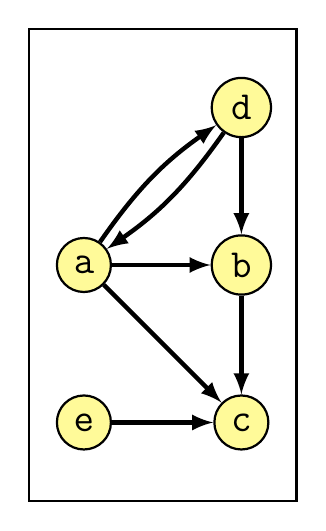
\begin{tikzpicture}[scale=1.00,transform shape]
%
\node[mynode] at (0, 0) (e) {e};
\node[mynode] at (2, 0) (c) {c};
\node[mynode] at (2, 2) (b) {b};
\node[mynode] at (0, 2) (a) {a};
\node[mynode] at (2, 4) (d) {d};
%
\draw[edgen] (a) edge node {} (b);
\draw[edgen] (a) edge node {} (c);
\draw[edgen] (e) edge node {} (c);
\draw[edgen] (a) edge[bend left=10] node {} (d);
\draw[edgen] (d) edge[bend left=10] node {} (a);
\draw[edgen] (d) edge node {} (b);
\draw[edgen] (b) edge node {} (c);

\path[draw=black,thick] (-0.7,-1.00) rectangle (2.7, 5.0);

\end{tikzpicture}

\newpage

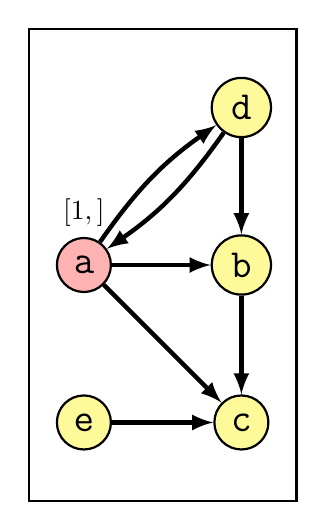
\begin{tikzpicture}[scale=1.00,transform shape]
%
\node[mynoder, label={above:$[1, ]$}] at (0, 2) (a) {a};
\node[mynode] at (2, 2) (b) {b};
\node[mynode] at (2, 0) (c) {c};
\node[mynode] at (2, 4) (d) {d};
\node[mynode] at (0, 0) (e) {e};
%
\draw[edgen] (a) edge node {} (b);
\draw[edgen] (a) edge node {} (c);
\draw[edgen] (e) edge node {} (c);
\draw[edgen] (a) edge[bend left=10] node {} (d);
\draw[edgen] (d) edge[bend left=10] node {} (a);
\draw[edgen] (d) edge node {} (b);
\draw[edgen] (b) edge node {} (c);

\path[draw=black,thick] (-0.7,-1.00) rectangle (2.7, 5.0);

\end{tikzpicture}

\newpage

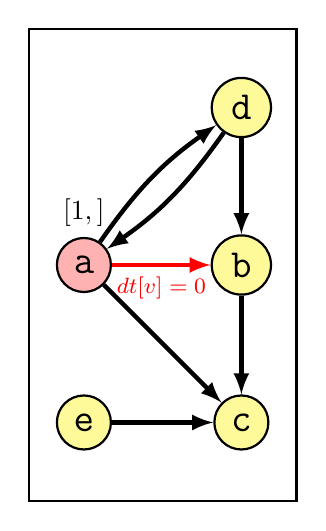
\begin{tikzpicture}[scale=1.00,transform shape]
%
\node[mynoder, label={above:$[1, ]$}] at (0, 2) (a) {a};
\node[mynode] at (2, 2) (b) {b};
\node[mynode] at (2, 0) (c) {c};
\node[mynode] at (2, 4) (d) {d};
\node[mynode] at (0, 0) (e) {e};
%
\draw[edger] (a) edge[below] node {\footnotesize $dt[v]=0$} (b);
\draw[edgen] (a) edge node {} (c);
\draw[edgen] (e) edge node {} (c);
\draw[edgen] (a) edge[bend left=10] node {} (d);
\draw[edgen] (d) edge[bend left=10] node {} (a);
\draw[edgen] (d) edge node {} (b);
\draw[edgen] (b) edge node {} (c);

\path[draw=black,thick] (-0.7,-1.00) rectangle (2.7, 5.0);

\end{tikzpicture}

\newpage

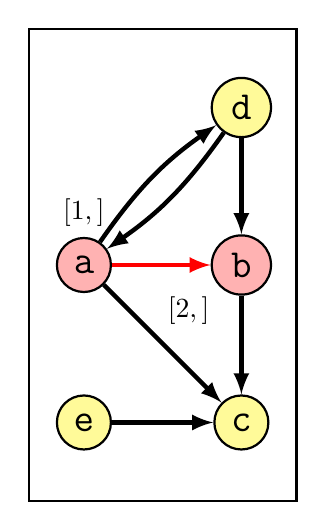
\begin{tikzpicture}[scale=1.00,transform shape]
%
\node[mynoder, label={above:$[1, ]$}] at (0, 2) (a) {a};
\node[mynoder, label={below left:$[2, ]$}] at (2, 2) (b) {b};
\node[mynode] at (2, 0) (c) {c};
\node[mynode] at (2, 4) (d) {d};
\node[mynode] at (0, 0) (e) {e};
%
\draw[edger] (a) edge node {} (b);
\draw[edgen] (a) edge node {} (c);
\draw[edgen] (e) edge node {} (c);
\draw[edgen] (a) edge[bend left=10] node {} (d);
\draw[edgen] (d) edge[bend left=10] node {} (a);
\draw[edgen] (d) edge node {} (b);
\draw[edgen] (b) edge node {} (c);

\path[draw=black,thick] (-0.7,-1.00) rectangle (2.7, 5.0);

\end{tikzpicture}

\newpage

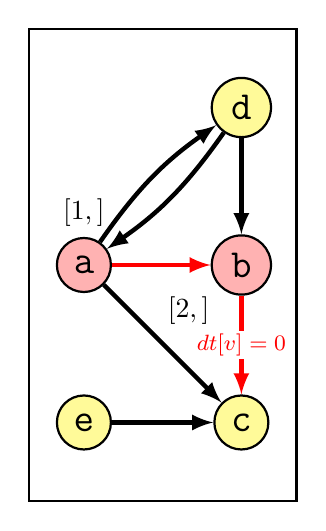
\begin{tikzpicture}[scale=1.00,transform shape]
%
\node[mynoder, label={above:$[1, ]$}] at (0, 2) (a) {a};
\node[mynoder, label={below left:$[2, ]$}] at (2, 2) (b) {b};
\node[mynode] at (2, 0) (c) {c};
\node[mynode] at (2, 4) (d) {d};
\node[mynode] at (0, 0) (e) {e};
%
\draw[edger] (a) edge node {} (b);
\draw[edgen] (a) edge node {} (c);
\draw[edgen] (e) edge node {} (c);
\draw[edgen] (a) edge[bend left=10] node {} (d);
\draw[edgen] (d) edge[bend left=10] node {} (a);
\draw[edgen] (d) edge node {} (b);
\draw[edger] (b) edge node[fill=white,rounded corners=2pt,inner sep=1pt] {\footnotesize $dt[v]=0$} (c);

\path[draw=black,thick] (-0.7,-1.00) rectangle (2.7, 5.0);

\end{tikzpicture}

\newpage

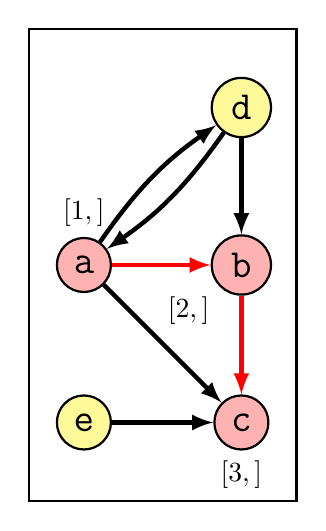
\begin{tikzpicture}[scale=1.00,transform shape]
%
\node[mynoder, label={above:$[1, ]$}] at (0, 2) (a) {a};
\node[mynoder, label={below left:$[2, ]$}] at (2, 2) (b) {b};
\node[mynoder, label={below:$[3, ]$}] at (2, 0) (c) {c};
\node[mynode] at (2, 4) (d) {d};
\node[mynode] at (0, 0) (e) {e};
%
\draw[edger] (a) edge node {} (b);
\draw[edgen] (a) edge node {} (c);
\draw[edgen] (e) edge node {} (c);
\draw[edgen] (a) edge[bend left=10] node {} (d);
\draw[edgen] (d) edge[bend left=10] node {} (a);
\draw[edgen] (d) edge node {} (b);
\draw[edger] (b) edge node {} (c);

\path[draw=black,thick] (-0.7,-1.00) rectangle (2.7, 5.0);

\end{tikzpicture}

\newpage

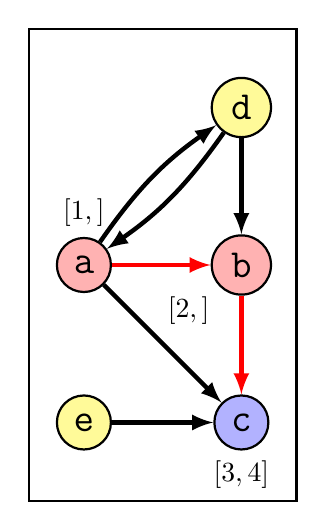
\begin{tikzpicture}[scale=1.00,transform shape]
%
\node[mynoder, label={above:$[1, ]$}] at (0, 2) (a) {a};
\node[mynoder, label={below left:$[2, ]$}] at (2, 2) (b) {b};
\node[mynodeb, label={below:$[3, 4]$}] at (2, 0) (c) {c};
\node[mynode] at (2, 4) (d) {d};
\node[mynode] at (0, 0) (e) {e};
%
\draw[edger] (a) edge node {} (b);
\draw[edgen] (a) edge node {} (c);
\draw[edgen] (e) edge node {} (c);
\draw[edgen] (a) edge[bend left=10] node {} (d);
\draw[edgen] (d) edge[bend left=10] node {} (a);
\draw[edgen] (d) edge node {} (b);
\draw[edger] (b) edge node {} (c);

\path[draw=black,thick] (-0.7,-1.00) rectangle (2.7, 5.0);

\end{tikzpicture}


\newpage

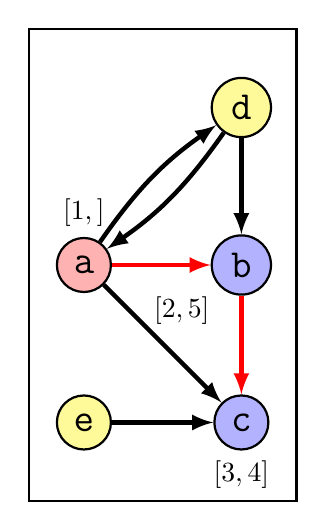
\begin{tikzpicture}[scale=1.00,transform shape]
%
\node[mynoder, label={above:$[1, ]$}] at (0, 2) (a) {a};
\node[mynodeb, label={below left:$[2, 5]$}] at (2, 2) (b) {b};
\node[mynodeb, label={below:$[3, 4]$}] at (2, 0) (c) {c};
\node[mynode] at (2, 4) (d) {d};
\node[mynode] at (0, 0) (e) {e};
%
\draw[edger] (a) edge node {} (b);
\draw[edgen] (a) edge node {} (c);
\draw[edgen] (e) edge node {} (c);
\draw[edgen] (a) edge[bend left=10] node {} (d);
\draw[edgen] (d) edge[bend left=10] node {} (a);
\draw[edgen] (d) edge node {} (b);
\draw[edger] (b) edge node {} (c);

\path[draw=black,thick] (-0.7,-1.00) rectangle (2.7, 5.0);

\end{tikzpicture}

\newpage

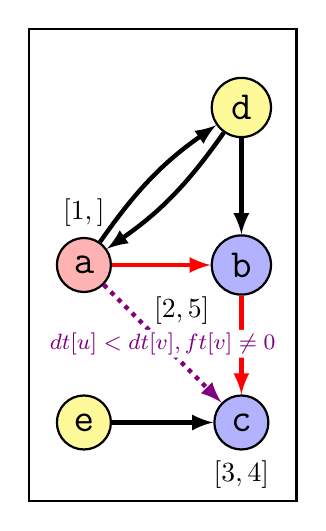
\begin{tikzpicture}[scale=1.00,transform shape]
%
\node[mynoder, label={above:$[1, ]$}] at (0, 2) (a) {a};
\node[mynodeb, label={below left:$[2, 5]$}] at (2, 2) (b) {b};
\node[mynodeb, label={below:$[3, 4]$}] at (2, 0) (c) {c};
\node[mynode] at (2, 4) (d) {d};
\node[mynode] at (0, 0) (e) {e};
%
\draw[edger] (a) edge node {} (b);
\draw[edgen] (e) edge node {} (c);
\draw[edgen] (a) edge[bend left=10] node {} (d);
\draw[edgen] (d) edge[bend left=10] node {} (a);
\draw[edgen] (d) edge node {} (b);
\draw[edger] (b) edge node {} (c);
\draw[edgevd] (a) edge node[fill=white,rounded corners=2pt,inner sep=1pt] {\footnotesize$dt[u]< dt[v], ft[v] \neq 0$} (c);

\path[draw=black,thick] (-0.7,-1.00) rectangle (2.7, 5.0);

\end{tikzpicture}

\newpage

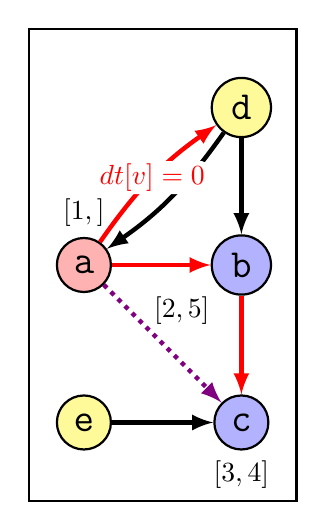
\begin{tikzpicture}[scale=1.00,transform shape]
%
\node[mynoder, label={above:$[1, ]$}] at (0, 2) (a) {a};
\node[mynodeb, label={below left:$[2, 5]$}] at (2, 2) (b) {b};
\node[mynodeb, label={below:$[3, 4]$}] at (2, 0) (c) {c};
\node[mynode] at (2, 4) (d) {d};
\node[mynode] at (0, 0) (e) {e};
%
\draw[edger] (a) edge node {} (b);
\draw[edgevd] (a) edge node {} (c);
\draw[edgen] (e) edge node {} (c);
\draw[edgen] (d) edge[bend left=10] node {} (a);
\draw[edgen] (d) edge node {} (b);
\draw[edger] (b) edge node {} (c);
\draw[edger] (a) edge[bend left=10] node[fill=white,rounded corners=2pt,inner sep=1pt] {$dt[v]=0$} (d);

\path[draw=black,thick] (-0.7,-1.00) rectangle (2.7, 5.0);

\end{tikzpicture}

\newpage

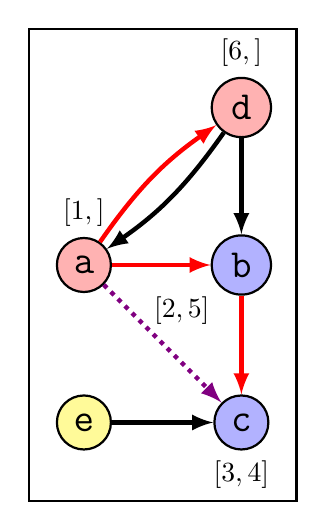
\begin{tikzpicture}[scale=1.00,transform shape]
%
\node[mynoder, label={above:$[1, ]$}] at (0, 2) (a) {a};
\node[mynodeb, label={below left:$[2, 5]$}] at (2, 2) (b) {b};
\node[mynodeb, label={below:$[3, 4]$}] at (2, 0) (c) {c};
\node[mynoder, label={above:$[6, ]$}] at (2, 4) (d) {d};
\node[mynode] at (0, 0) (e) {e};
%
\draw[edger] (a) edge node {} (b);
\draw[edgevd] (a) edge node {} (c);
\draw[edgen] (e) edge node {} (c);
\draw[edger] (a) edge[bend left=10,above left] node {} (d);
\draw[edgen] (d) edge[bend left=10] node {} (a);
\draw[edgen] (d) edge node {} (b);
\draw[edger] (b) edge node {} (c);

\path[draw=black,thick] (-0.7,-1.00) rectangle (2.7, 5.0);

\end{tikzpicture}

\newpage

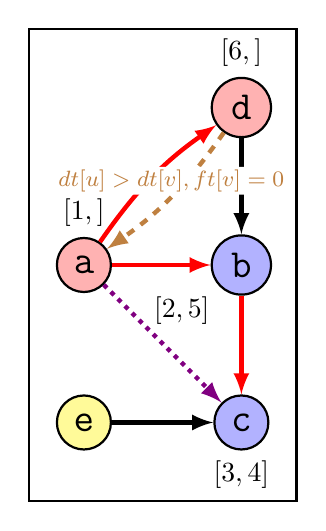
\begin{tikzpicture}[scale=1.00,transform shape]
%
\node[mynoder, label={above:$[1, ]$}] at (0, 2) (a) {a};
\node[mynodeb, label={below left:$[2, 5]$}] at (2, 2) (b) {b};
\node[mynodeb, label={below:$[3, 4]$}] at (2, 0) (c) {c};
\node[mynoder, label={above:$[6, ]$}] at (2, 4) (d) {d};
\node[mynode] at (0, 0) (e) {e};
%
\draw[edger] (a) edge node {} (b);
\draw[edgevd] (a) edge node {} (c);
\draw[edgen] (e) edge node {} (c);
\draw[edger] (a) edge[bend left=10,above left] node {} (d);
\draw[edgen] (d) edge node {} (b);
\draw[edger] (b) edge node {} (c);
\draw[edgegd] (d) edge[bend left=10, above] node[fill=white,rounded corners=2pt,inner sep=1pt] {\footnotesize $dt[u] > dt[v], ft[v] = 0$} (a);

\path[draw=black,thick] (-0.7,-1.00) rectangle (2.7, 5.0);

\end{tikzpicture}

\newpage

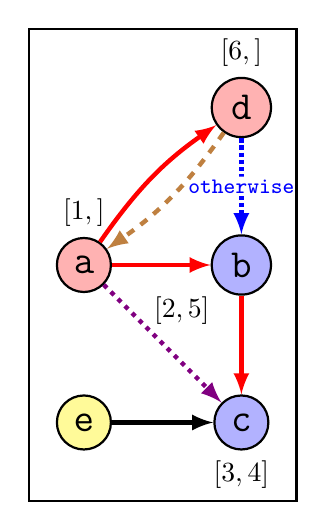
\begin{tikzpicture}[scale=1.00,transform shape]
%
\node[mynoder, label={above:$[1, ]$}] at (0, 2) (a) {a};
\node[mynodeb, label={below left:$[2, 5]$}] at (2, 2) (b) {b};
\node[mynodeb, label={below:$[3, 4]$}] at (2, 0) (c) {c};
\node[mynoder, label={above:$[6, ]$}] at (2, 4) (d) {d};
\node[mynode] at (0, 0) (e) {e};
%
\draw[edgexd] (d) edge node[fill=white,rounded corners=2pt,inner sep=1pt] {\footnotesize otherwise} (b);
\draw[edger] (a) edge node {} (b);
\draw[edgevd] (a) edge node {} (c);
\draw[edgen] (e) edge node {} (c);
\draw[edger] (a) edge[bend left=10] node {} (d);
\draw[edgegd] (d) edge[bend left=10] node {} (a);
\draw[edger] (b) edge node {} (c);

\path[draw=black,thick] (-0.7,-1.00) rectangle (2.7, 5.0);

\end{tikzpicture}

\newpage

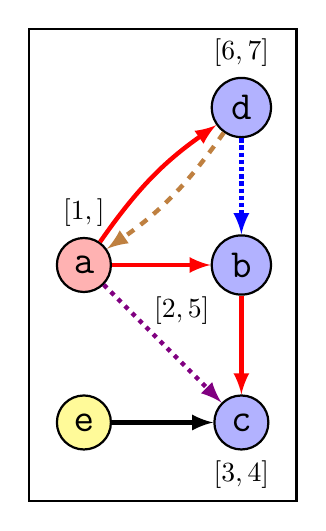
\begin{tikzpicture}[scale=1.00,transform shape]
%
\node[mynoder, label={above:$[1, ]$}] at (0, 2) (a) {a};
\node[mynodeb, label={below left:$[2, 5]$}] at (2, 2) (b) {b};
\node[mynodeb, label={below:$[3, 4]$}] at (2, 0) (c) {c};
\node[mynodeb, label={above:$[6, 7]$}] at (2, 4) (d) {d};
\node[mynode] at (0, 0) (e) {e};
%
\draw[edger] (a) edge node {} (b);
\draw[edgevd] (a) edge node {} (c);
\draw[edgen] (e) edge node {} (c);
\draw[edger] (a) edge[bend left=10] node {} (d);
\draw[edgegd] (d) edge[bend left=10] node {} (a);
\draw[edgexd] (d) edge node {} (b);
\draw[edger] (b) edge node {} (c);

\path[draw=black,thick] (-0.7,-1.00) rectangle (2.7, 5.0);

\end{tikzpicture}

\newpage

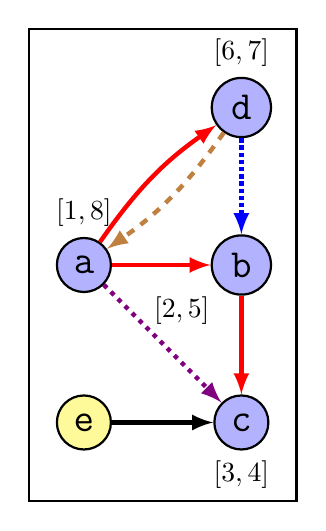
\begin{tikzpicture}[scale=1.00,transform shape]
%
\node[mynodeb, label={above:$[1, 8]$}] at (0, 2) (a) {a};
\node[mynodeb, label={below left:$[2, 5]$}] at (2, 2) (b) {b};
\node[mynodeb, label={below:$[3, 4]$}] at (2, 0) (c) {c};
\node[mynodeb, label={above:$[6, 7]$}] at (2, 4) (d) {d};
\node[mynode] at (0, 0) (e) {e};
%
\draw[edger] (a) edge node {} (b);
\draw[edgevd] (a) edge node {} (c);
\draw[edgen] (e) edge node {} (c);
\draw[edger] (a) edge[bend left=10] node {} (d);
\draw[edgegd] (d) edge[bend left=10] node {} (a);
\draw[edgexd] (d) edge node {} (b);
\draw[edger] (b) edge node {} (c);

\path[draw=black,thick] (-0.7,-1.00) rectangle (2.7, 5.0);

\end{tikzpicture}

\newpage

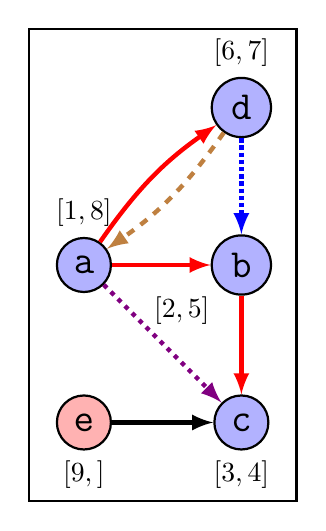
\begin{tikzpicture}[scale=1.00,transform shape]
%
\node[mynodeb, label={above:$[1, 8]$}] at (0, 2) (a) {a};
\node[mynodeb, label={below left:$[2, 5]$}] at (2, 2) (b) {b};
\node[mynodeb, label={below:$[3, 4]$}] at (2, 0) (c) {c};
\node[mynodeb, label={above:$[6, 7]$}] at (2, 4) (d) {d};
\node[mynoder, label={below:$[9, ]$}] at (0, 0) (e) {e};
%
\draw[edger] (a) edge node {} (b);
\draw[edgevd] (a) edge node {} (c);
\draw[edgen] (e) edge node {} (c);
\draw[edger] (a) edge[bend left=10] node {} (d);
\draw[edgegd] (d) edge[bend left=10] node {} (a);
\draw[edgexd] (d) edge node {} (b);
\draw[edger] (b) edge node {} (c);

\path[draw=black,thick] (-0.7,-1.00) rectangle (2.7, 5.0);

\end{tikzpicture}

\newpage

\begin{tikzpicture}[scale=1.00,transform shape]
%
\draw[edgexd] (e) edge[below] node[fill=white,rounded corners=2pt,inner sep=1pt] {\footnotesize otherwise} (c);
\node[mynodeb, label={above:$[1, 8]$}] at (0, 2) (a) {a};
\node[mynodeb, label={below left:$[2, 5]$}] at (2, 2) (b) {b};
\node[mynodeb, label={below:$[3, 4]$}] at (2, 0) (c) {c};
\node[mynodeb, label={above:$[6, 7]$}] at (2, 4) (d) {d};
\node[mynoder, label={below:$[9, ]$}] at (0, 0) (e) {e};
%
\draw[edger] (a) edge node {} (b);
\draw[edgevd] (a) edge node {} (c);
\draw[edger] (a) edge[bend left=10] node {} (d);
\draw[edgegd] (d) edge[bend left=10] node {} (a);
\draw[edgexd] (d) edge node {} (b);
\draw[edger] (b) edge node {} (c);

\path[draw=black,thick] (-0.7,-1.00) rectangle (2.7, 5.0);

\end{tikzpicture}

\newpage

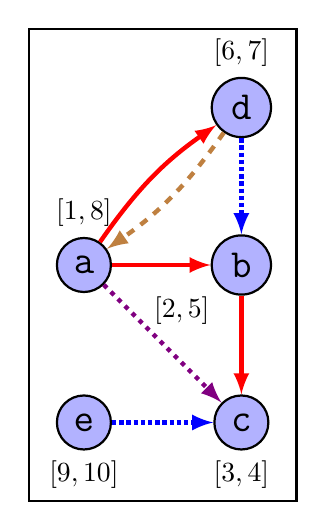
\begin{tikzpicture}[scale=1.00,transform shape]
%
\node[mynodeb, label={above:$[1, 8]$}] at (0, 2) (a) {a};
\node[mynodeb, label={below left:$[2, 5]$}] at (2, 2) (b) {b};
\node[mynodeb, label={below:$[3, 4]$}] at (2, 0) (c) {c};
\node[mynodeb, label={above:$[6, 7]$}] at (2, 4) (d) {d};
\node[mynodeb, label={below:$[9, 10]$}] at (0, 0) (e) {e};
%
\draw[edger] (a) edge node {} (b);
\draw[edgevd] (a) edge node {} (c);
\draw[edgexd] (e) edge node {} (c);
\draw[edger] (a) edge[bend left=10] node {} (d);
\draw[edgegd] (d) edge[bend left=10] node {} (a);
\draw[edgexd] (d) edge node {} (b);
\draw[edger] (b) edge node {} (c);

\path[draw=black,thick] (-0.7,-1.00) rectangle (2.7, 5.0);

\end{tikzpicture}

\end{document}




















